\chapter{}

\section{Эллипс (продолжение)}

\begin{theorem}
    $$ (x_0, y_0) \text{ лежит на эллипсе } \frac{x^2}{a^2} + \frac{y^2}{b^2} = 1 $$
    $$ \implies \text{касательная в точке } (x_0, y_0) \text{ выражается формулой } \frac{xx_0}{a^2} + \frac{yy_0}{b^2} = 1 $$
\end{theorem}

\begin{proof}
	Прямая проходит через точку $(x_0, y_0) $
    $$ A = \frac{x_0}{a^2} \qquad B = \frac{y_0}{b^2} \qquad C = -1 $$
    $$ A^2 a^2 + B^2 b^2 = \frac{x_0^2}{a^2} a^2 + \frac{y_0^2}{b^2} b^2 = 1 = C ^2 $$
\end{proof}

\begin{theorem}[Оптическое свойтсво эллипса]
    $ F_1, F_2 $ -- фокусы, $ M $ -- точка на эллипсе, $ \vec{n} $ -- вектор нормали к касательной в точке $M$
    $$ \implies \angle (\vect{F_1M}; \vec{n}) = \angle (\vect{F_2M}; \vec{n}) $$
\end{theorem}

\begin{proof}
    $$ \frac{xx_0}{a^2} + \frac{yy_0}{b^2} = 1 $$
    $$ \vec{n} = \frac{x_0}{a^2}; \frac{y_0}{b^2}) $$
    $$ \vect{F_1M} = (x_0 + c; y_0) $$
    $$ \vect{F_2M} = (x_0 - c; y_0) $$
    $$ \frac{(x_0 + c; y_0) \cdot (\frac{x_0}{a^2}; \frac{y_0}{a^2})}{|F_1M| \cdot |M|} \stackrel?= \frac{(x_0 - c; y_0) \cdot (\frac{x_0}{a^2}; \frac{y_0}{b^2})}{|F_2M| \cdot |M|} $$
    $$ \frac{\frac{x_0^2}{a^2} + \frac{cx_0}{a^2} + \frac{y_0^2}{b^2}}{a + ex_0} \stackrel?= \frac{\frac{x_0^2}{a^2} - \frac{cx_0}{a^2} + \frac{y_0^2}{b^2}}{a - ex_0} $$
    $$ \frac{1 + \frac{ex_0}a}{a + ex_0} \stackrel?= \frac{1 - \frac{ex_0}a}{a - ex_0} $$
    $$ \frac1a = \frac 1a $$
\end{proof}

\section{Гипербола}

\begin{definition}
	ГМТ $ M : |F_1M - f_2M| = 2a $ называется гиперболой
\end{definition}

\begin{definition}
    ГМТ $ M : \frac{FM}{|M, l|} = e > 1 $ называется гиперболой. $ e $ называется эксцентриситетом
\end{definition}

\begin{definition}
    В подходящих координатах гипербола задаётся как $ \frac{x^2}{a^2} - \frac{y^2}{b^2} = 1 $
\end{definition}

\begin{theorem}
	Все три определения равносильны
\end{theorem}

\begin{figure}[h]
    \centering
    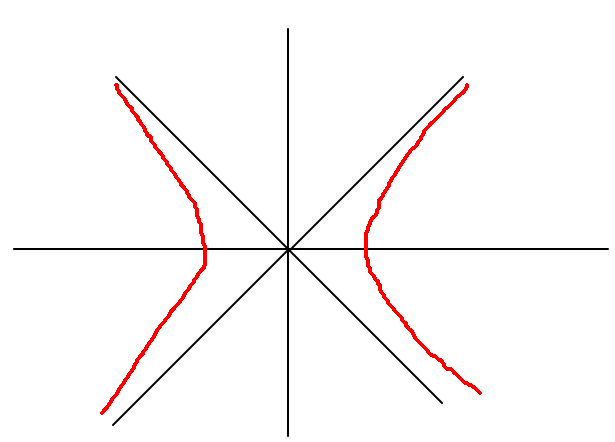
\includegraphics[scale=0.5]{1}
    \caption{Гипербола}
\end{figure}

\begin{statement}
    Асимптоты: $ y = \pm \frac{b}a x $
\end{statement}

\begin{proof}
    $$ y = \pm b \sqrt{ -1 + \frac{x^2}{a^2}} $$
    $$ \limi{x} \frac{ \pm b \sqrt{\frac{x^2}{a^2} - 1}}x = \limi{x} \sqrt{\frac{x^2 - a^2}{x^2}} $$
    $$ l = \limi{x} (\pm b \sqrt{\frac{x^2}{a^2} - 1} \mp \frac{b}a x) = \pm \frac{b}a \limi{x} (\sqrt{x^2 - a^2} - x) = \pm \frac{b}a \limi{x} \frac{-a}{\sqrt{x^2 - a^2} + x} $$
\end{proof}

\begin{theorem}
    $ Ax + By + C = 0 $ касается в точке $ (x_0, y_0) $ гиперболы $ \frac{x^2}{a^2} + \frac{y^2}{b^2} = 1 $, то
    $$ \frac{x^2}{a^2} - \frac{y^2}{b^2} = 1 \iff A^2a^2 - B^2b^2 = C^2 $$
\end{theorem}

\begin{theorem}[Оптическое свойство гиперболы]
    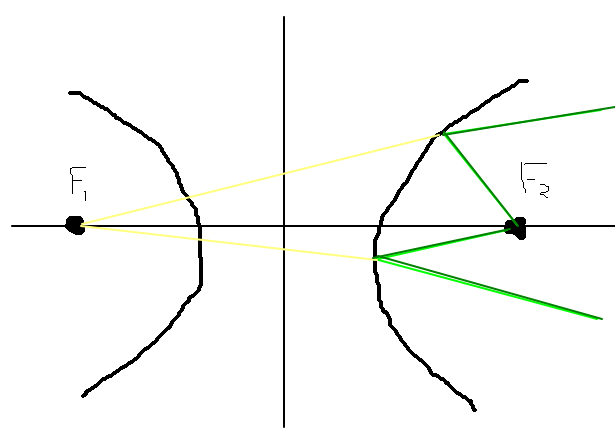
\includegraphics[scale=0.4]{2}
\end{theorem}

\begin{lemma}
	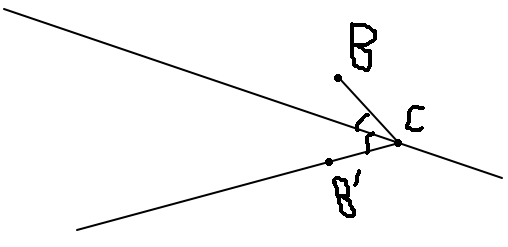
\includegraphics[scale=0.4]{3}
    $$ |AC - BC | \to \max $$
    $$ |AC - B'C | \le AB' $$
\end{lemma}

\section{Парабола}

\begin{definition}
	Есть точка $F$ и  прямая $l$ \\
    ГМТ $ M : \frac{FM}{|M, l|} = l = 1 $ называется параболой
\end{definition}

\begin{definition}
	В подходящих координатах парабола задаётся как $ y^2 = 2px $
\end{definition}

\begin{figure}[h]
    \centering
    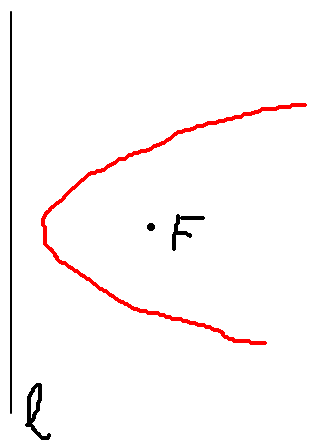
\includegraphics[scale=0.5]{4}
    \caption{Парабола}
\end{figure}

Фокус $F (\frac{p}2; 0) $, $ l : x = - \frac{p}2 $

\begin{theorem}
	Определения равносильны
\end{theorem}

\begin{proof}
    $$ F(\frac{p}2) \qquad l: x = - \frac{p}2 \qquad M (x, y) $$
    $$ FM = \sqrt{(x - \frac{p}2)^2 + y^2} \stackrel?= |M, l| = x + \frac{p}2 $$
    $$ x^2 - px + \frac{p^2}4 + y^2 = x^2 + px + \frac{p^2}4 $$
    $$ y^2 = 2px $$
\end{proof}
